\documentclass[titlepage]{report}
\usepackage[utf8]{inputenc}
\usepackage[OT1]{fontenc}
\usepackage{cmbright}
\usepackage{amsmath}
\usepackage{fancyhdr}
\usepackage{parskip}
\usepackage{amssymb}
\usepackage{centernot}
\usepackage{tikz}
\usepackage{subcaption}
\usepackage{amsthm}
\usepackage{cancel}

% info --------------------------------

\title{Causal Networks}
\author{Giuseppe Magazzù}
\date{2021 - 2022}

% fancyhdr ----------------------------

\pagestyle{fancy}
\setlength{\headheight}{13pt}
\cfoot{\thepage}
\lhead{}
\rhead{\leftmark}

\renewcommand{\headrulewidth}{0.1pt}
\renewcommand{\footrulewidth}{0pt}

% custom ------------------------------

% src: https://tex.stackexchange.com/questions/164338/looking-for-a-specific-symbol-used-in-set-theory-cant-find-on-detexify

\makeatletter
\DeclareRobustCommand{\ind}{%
  \mathbin{\mathpalette\var@malg\perp}%
}

\newcommand\var@malg[2]{%
  \rlap{$\m@th#1#2$}\mkern6mu{#1#2}%
}
\makeatother

\newcommand{\nind}{\centernot\ind}

% document ----------------------------

\begin{document}

\maketitle

\pagenumbering{roman}

\tableofcontents

\clearpage
\pagenumbering{arabic}


\chapter{The Potential Outcome Framework}

Fundamental Problem of Causal Inference:
\begin{itemize}
  \item Average Treatment Effects and Missing Data Interpretation
  \item Ignorability - Exchangeability
  \item Conditional Exchangeability - Uncounfoundedness
  \item Positivity - Overlap - Common Support and Extrapolation
  \item No interference, Consistency, SUTVA
\end{itemize}

\section{Potential Outcome}

\begin{itemize}
  \item $X$ \textbf{Treatment} variabile aleatoria
  \item $Y$ \textbf{Outcome} variabile aleatoria
  \item $Z$ \textbf{Covariate} insieme di variabili aleatorie
\end{itemize}

Il \textbf{potential outcome} $Y(x)$ denota quale sarebbe l'\textbf{outcome} quando $X = x$, ovvero se il treatment che è stato scelto è $x$.
Una volta che viene osservato il \textbf{potential outcome} Y(x) questo assume valore Y chiamato \textbf{outcome}.

Una \textbf{popolazione} consiste di molti individui o unità.
Ogni individuio (unità) è associato a uno o più variabili $Z$ \textbf{covariate}.

Denotiamo $X$, $Y$, $Z$ dell'individuio $i$-esimo come $X_i$, $Y_i$, $Z_i$.

$Y(x)$ è una variabile aleatoria\\
$Y_i(x)$ non è trattata come una variabile aleatoria poiché specifica per l'individuo

\subsection*{Individual Treatment Effect (ITE)}
Per verificare se c'è una relazione causale tra $X$ e $Y$ si può calcolare la seguente differenza
$\tau_i \triangleq Y_i(1) - Y_i(0)$.

Se il potential outcome è uguale in entrambi i casi ($\tau_i = 0$) allora non c'è relazione causale.
Nel caso contrario si può notare che diversi treatment portano a diversi outcome e quindi c'è una relazione causale.

Non possiamo osservare tutti i \textbf{potential outcome} poiché l'osservarne uno influenzerebbe gli altri.
I \textbf{potential outcome} che non possono essere osservati vengono chiamati \textbf{counterfactual}, mentre quello che osserviamo è il \textbf{factual}.
%
\begin{flalign*}
  &Y(1) = \; ? \quad\Rightarrow\quad Y=0, X=1 \quad\Rightarrow\quad Y(1) = \; ? \qquad \text{counterfactual}&\\
  &Y(0) = \; ? \quad\Rightarrow\quad Y=0, X=0 \quad\Rightarrow\quad Y(0) = 1 \qquad \text{factual}&
\end{flalign*}

\subsection*{Average Treatment Effect (ATE)}
$\tau \triangleq \mathbb{E}[Y_i(1) - Y_i(0)]$

\chapter{Flow of Associations and Causal Graphs}

In un grafo diretto indichiamo con $pa(X)$ i \textbf{genitori} del nodo $X$ e $ch(Y)$ i \textbf{figli} del nodo $Y$.

\begin{center}
  \begin{minipage}[c]{0.5\linewidth}
    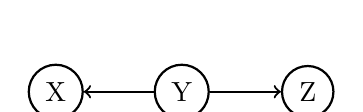
\begin{tikzpicture}[node distance={16mm}, thick, main/.style = {draw, circle}]
      \node[main] (1) {X};
      \node[main] (2) [right of=1] {Y};
      \node[main] (3) [right of=2] {Z};
      \draw[<-] (1) -- (2);
      \draw[->] (2) -- (3);
    \end{tikzpicture}
  \end{minipage}
  %
  \begin{minipage}[c]{0.4\linewidth}
    \setlength{\abovedisplayskip}{0pt}
    \begin{flalign*}
      &pa(Y) = \emptyset&  ch(Y) &= \{X,Z\}&\\
      &pa(X) = Y& ch(X) &= \emptyset&
    \end{flalign*}
  \end{minipage}
\end{center}

Un \textbf{cammino} è una qualsiasi sequenza di nodi adiacenti, indipendentemente dalla direzione degli archi che li collega.

Un \textbf{cammino diretto} è un qualsiasi \textbf{cammino} tra due nodi in cui tutti gli archi che li collega hanno la stessa direzione.

$de(Y)$ è l'insieme dei nodi \textbf{discendenti} del nodo $Y$, ovvero tutti i nodi che possono essere raggiunti da $Y$.

$an(Z)$ è l'insieme dei nodi \textbf{antenati} del nodo $Z$, ovvero tutti i nodi che da $Z$ possono essere raggiunti.

\begin{center}
  \begin{minipage}[c]{0.4\linewidth}
    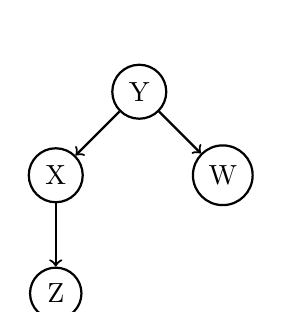
\begin{tikzpicture}[node distance={15mm}, thick, main/.style = {draw, circle}]
      \node[main] (1) {Y};
      \node[main] (2) [below left of=1] {X};
      \node[main] (3) [below right of=1] {W};
      \node[main] (4) [below of=2] {Z};
      \draw[->] (1) -- (2);
      \draw[->] (1) -- (3);
      \draw[->] (2) -- (4);
    \end{tikzpicture}
  \end{minipage}
  \begin{minipage}[c]{0.3\linewidth}
    $an(Z) = \{X, Y\}$\\
    $an(Y) = \emptyset$

    \bigskip
    $de(Y) = \{X, Z, W\}$\\
    $de(W) = \emptyset$
  \end{minipage}
\end{center}

\section{Bayesian Networks}
In una rete bayesiana vogliamo modellare la distribuzione di probabilità $P(X_1, \dots, X_n)$.
Tramite la \textbf{Chain Rule} possiamo riscriverla nel seguente modo:
\begin{flalign*}
  P(X_1, \dots, X_n) &= P(X_1)P(X_2|X_1)P(X_3|X_1,X_2) \cdot\cdot\cdot P(X_n|X_1, \dots, X_{n-1}) & \\
  &= P(X_1)\prod_{i=2}^n{P(X_i|X_1, \dots, X_{i-1})} &
\end{flalign*}
%
\textbf{Local Markov Assumption}:
Un nodo $X$ è indipendente da tutti i suoi non-discendenti date l'evidenze di tutti i nodi genitori $pa(X)$.

Data questa assunzione possiamo applicare la fattorizzazione della probabilità $P$.
\begin{flalign*}
  &P(X_1, \dots, X_n) = \prod_{i=1}^n{P(X_i|pa(X_i)})&
\end{flalign*}
%
In questo modo possiamo ridurre il numero di parametri della rete.

Una distribuzione di probabilità $P$ si dice che sia Markov se ogni nodo $X$ rispetta la Local Markov Assumption.

L'assunzione di Markov non ci da informazioni riguardo relazioni di dipendenza tra i nodi.
Quindi estendiamo quest'assunzione.

\textbf{Minimality Assumption}
\begin{itemize}
  \item Dato $pa(X)$, un nodo $X$ è indipendente da tutti i suoi non-discendenti.
  \item I nodi adiacenti sono dipendenti.
\end{itemize}

Dato un DAG $G$, se $P$ è Markov allora sappiamo:
\begin{itemize}
  \item $P$ soddisfa un insieme di indipendenze specificate dalla struttura di $G$.
  \item se $P$ soddisfa pure la Minimality Assumption, allora l'insieme di indipendenze è minimale,
        ovvero $P$ non soddisfa altre indipendenze in $G$.
        Questo equivale a dire che tutti i nodi adiacenti sono dipendenti.
\end{itemize}

\section{Causal Networks}

Una variabile $X$ si dice \textbf{causa} di una variabile $Y$ se $Y$ può
cambiare in risposta a un cambiamento di $X$.

\textbf{Causal Edge Assumption}:
Ogni variabile associata a un nodo è causata dalle variabili dei nodi genitori.

Un \textbf{Grafo Causale} è un DAG in cui è soddisfatta la proprietà \textbf{Causal Edge Assumption}.

\begin{center}
  \begin{minipage}[c]{0.3\linewidth}
    \vspace{0pt}\
    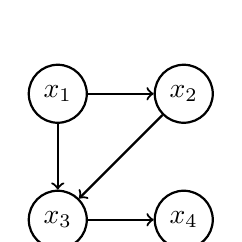
\begin{tikzpicture}[node distance={16mm}, thick, main/.style = {draw, circle}]
      \node[main] (1) {$x_1$};
      \node[main] (2) [right of=1] {$x_2$};
      \node[main] (3) [below of=1] {$x_3$};
      \node[main] (4) [right of=3] {$x_4$};
      \draw[->] (1) -- (2);
      \draw[->] (1) -- (3);
      \draw[->] (2) -- (3);
      \draw[->] (3) -- (4);
    \end{tikzpicture}
  \end{minipage}
  %
  \begin{minipage}[c]{0.4\linewidth}
    $X_1$ causa direttamente $X_2$ e $X_3$\\
    $X_2$ causa direttamente $X_3$\\
    $X_3$ causa direttamente $X_4$

    \bigskip
    $X_1$ causa indirettamente $X_4$
  \end{minipage}
\end{center}
\bigskip

Per capire la differenza tra association flow e causation flow utilizziamo dei grafi elementari.

\begin{figure}[h]
  \centering

  \begin{subfigure}[c]{0.34\linewidth}
    \centering
    \bigskip
    \bigskip
    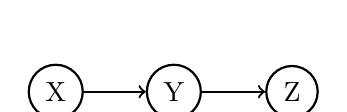
\begin{tikzpicture}[node distance={15mm}, thick, main/.style = {draw, circle}]
      \node[main] (1) {X};
      \node[main] (2) [right of=1] {Y};
      \node[main] (3) [right of=2] {Z};
      \draw[->] (1) -- (2);
      \draw[->] (2) -- (3);
    \end{tikzpicture}
    \bigskip
    \caption{Chain}
  \end{subfigure}
  %
  \begin{subfigure}[c]{0.32\linewidth}
    \centering
    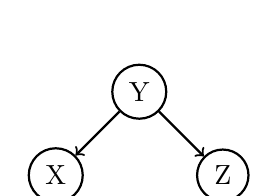
\begin{tikzpicture}[node distance={15mm}, thick, main/.style = {draw, circle}]
      \node[main] (2) {Y};
      \node[main] (1) [below left of=2] {X};
      \node[main] (3) [below right of=2] {Z};
      \draw[->] (2) -- (1);
      \draw[->] (2) -- (3);
    \end{tikzpicture}
    \caption{Fork}
  \end{subfigure}
  %  
  \begin{subfigure}[c]{0.32\linewidth}
    \centering
    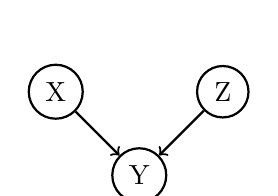
\begin{tikzpicture}[node distance={15mm}, thick, main/.style = {draw, circle}]
      \node[main] (2) {Y};
      \node[main] (1) [above left of=2] {X};
      \node[main] (3) [above right of=2] {Z};
      \draw[->] (1) -- (2);
      \draw[->] (3) -- (2);
    \end{tikzpicture}
    \caption{Collider}
  \end{subfigure}
\end{figure}

Il flusso di associazione esprime che due nodi del grafo sono associati o meno.

Vogliamo sapere se due nodi sono (statisticamente) dipendenti o indipendenti.

\subsubsection*{Un-connected Nodes}
Due nodi sconnessi non sono associati. Questo può essere dimostrato applicando la fattorizzazione.
%
\begin{align*}
  P(X, Y) & = P(X | Y) P(Y)             \qquad & \text{(probabilità composta)} \\
          & = P(X | pa(X)) P(Y | pa(Y)) \qquad & \text{(fattorizzazione)}      \\
          & = P(X) P(Y)                 \qquad & \text{indipendenza}
\end{align*}

Due nodi connessi adiacenti sono dipendenti per la \textbf{local edge assumption}.

\subsubsection*{Chain e Fork}


\subsubsection*{Collider}


\section{D-Separation}
Un percorso $p$ si dice bloccato da un insieme di nodi $S$ sse
\begin{itemize}
  \item $p$ contiene una chain $A \rightarrow B \rightarrow C$ o una fork $A \leftarrow B \rightarrow C$ e $B \in S$
  \item $p$ contiene un collider $A \rightarrow B \leftarrow C$ e $B \notin S, de(B) \nsubseteq S$
\end{itemize}
Se l'insieme $S$ blocca ogni percorso tra due nodi $X$ e $Y$, allora $X$ e $Y$ si dicono \textbf{d-separati} da $S$,
e quindi indipendenti dato $S$.

ESEMPI...

La d-separazione implica l'indipendenza condizionale.

\begin{itemize}
  \item Due variabili $X$ e $Y$ sono d-separate nel grafo $G$ \\quando condizionate dall'insieme $S$ ($X \ind_G Y | S$).
  \item Due variabili $X$ e $Y$ sono indipendenti nella distribuzione $p$ \\quando condizionate dall'insieme $S$ ($X \ind_p Y | S$).
\end{itemize}

$X \ind_G Y | S \Rightarrow X \ind_p Y | S$

\chapter{Causal Models}
In un \textbf{randomized control experiment} tutti i fattori $X_1, ..., X_n$ che influenzano l'outcome $Y$ sono statici o variati randomicamente tranne uno  $X_i$.
In questo modo un cambiamento nell'outcome $Y$ sarà dovuto solo da quel fattore $X_i$.

Spesso non è possibile effettuare gli esperimenti per cause pratiche o etiche, quindi si eseguono degli studi osservazionali in un cui
si raccolgono i dati rispetto ad alterarli.

Il problema degli studi osservazionali è distinguere la causazione dalla correlazione.

\section{Intervention and do-Operator}
\begin{center}
  \begin{minipage}{0.475\linewidth}
    \centering
    \textbf{Intervening}

    Cambiamo il sistema fissando $X=x$ e osserviamo i cambiamenti su tutta la popolazione.
  \end{minipage}
  \begin{minipage}{0.475\linewidth}
    \centering
    \textbf{Conditioning}

    Non cambiamo nulla e consideriamo un sottoinsieme della popolazione $X=x$.
  \end{minipage}
\end{center}

Denotiamo l'intervention con il do-operator $do(X=x)$.
\begin{align*}
  P(Y(x) = y) = P(Y = y | do(X = x)) = P(y | do(x))
\end{align*}
%
\begin{align*}
   & P(Y | X = x) = P(y | x)         \qquad & \text{observational distribution}  \\
   & P(Y | do(X = x)) = P(y | do(x)) \qquad & \text{interventional distribution}
\end{align*}

Un'espressione con $do$ è detta interventional expression, mentre senza $do$ è detta observational expression.

Un'interventional expression che può essere ridotta a una observational expression è detta \textbf{identificabile}.

Una stima è detta causale se contiene il do-operator, statistica altrimenti.

\bigskip
\begin{center}
  \begin{minipage}{0.475\linewidth}
    \centering
    \textbf{pre-intervention distribution}
    \begin{align*}
      P(Y | do(x), Z = z)
    \end{align*}
  \end{minipage}
  \begin{minipage}{0.475\linewidth}
    \centering
    \textbf{post-intervention distribution}
    \begin{align*}
      P(Y | x, Z = z)
    \end{align*}
  \end{minipage}
\end{center}
\bigskip

\section{Modularity and Adjustment Formula}
Il \textbf{causal mechanism} è un meccanismo che genera $X_i$ come distribuzione condizionale di $X_i$ dati i genitori (cause) $pa(X_i)$, ovvero $P(X_i | pa(X_i))$.

Assunzione: Le intervention sono locali

Un intervention su una variabile $X_i$ cambia solo il suo causal mechanism, non cambia il causal mechanism che genera un'altra variabile $X_j$.

\subsection*{Modularity - Independence Mechanism - Invariance}
Se interveniamo su un insieme di variabili $S$ fissando valori costanti,
allora per ogni variabile $X_i \in \{X_1, ..., X_n\}$ possiamo affermare che:
\begin{enumerate}
  \item Se $X_i \in S$, allora $P(X_i = x| pa(X_i)) = 1$ se $x$ è il valore assegnato dall'intervention $do(X_i=x)$, 0 altrimenti
  \item Se $X_i \not\in S$, allora $P(X_i = x | pa(X_i))$ rimane inalterato
\end{enumerate}

Data una variabile $X_i \in S$, un valore $x$ di $X_i$ è \textbf{consistente} con l'intervention su $X_i$ se $x$ è uguale al valore che è stato assegnato nell'intervention $do(X_i=x)$.

Una volta impostato il valore di $X_i$ non importa più il valore dei nodi genitori $pa(X_i)$, poiché al variare di $pa(X_i)$ non varierà il valore di $X_i$.

Questo possiamo rappresentarlo attraverso un grafo (detto manipulated graph o \textbf{post-intervention graph}) in cui si rimuoviamo gli archi entranti in $X_i$; se non ce ne sono, vuol dire che l'intervention non ha conseguenze sulla distribuzione post-intervention
$p(y|do(x)) = p(y|x)$.

\subsection*{Adjustment Formula}
Dato il seguente grafo causale e il suo corrispettivo grafo manipolato a seguito dell'intervention sulla variabile $X$.

\begin{center}
  \begin{minipage}{0.4\linewidth}
    \centering
    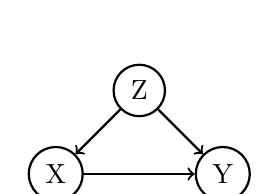
\begin{tikzpicture}[node distance={15mm}, thick, main/.style = {draw, circle}]
      \node[main] (1) {Z};
      \node[main] (2) [below right of=1] {Y};
      \node[main] (3) [below left of=1] {X};
      \draw[->] (1) -- (2);
      \draw[->] (1) -- (3);
      \draw[->] (3) -- (2);
    \end{tikzpicture}

    pre-intervention graph
  \end{minipage}
  %
  {\Large$\overset{do(X = x)}{\Longrightarrow}$}
  %
  \begin{minipage}{0.4\linewidth}
    \centering
    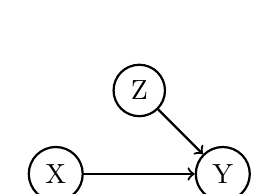
\begin{tikzpicture}[node distance={15mm}, thick, main/.style = {draw, circle}]
      \node[main] (1) {Z};
      \node[main] (2) [below right of=1] {Y};
      \node[main] (3) [below left of=1] {X};
      \draw[->] (1) -- (2);
      \draw[->] (3) -- (2);
    \end{tikzpicture}

    post-intervention graph
  \end{minipage}
\end{center}

Possiamo osservare sotto la condizione di \textbf{modularity assumption} che:
\begin{enumerate}
  \item $P(Y = y|do(X = x)) = Pm (Y = y|X = x)$
  \item $P(Z|do(X=x)) = P_m(Z|x) = P(Z)$
  \item $P(Y|do(X=x), Z) = P_m(Y|x,Z) = P(Y|x,Z)$
\end{enumerate}

La probabilità marginale $P(Z)$ e la probabilità condizionale $P(Y|x,Z)$ sono invarianti all'intervention.
Questo perché il causal mechanism di X non influenza il causal mechanism delle altre variabili.

Date le seguenti uguaglianze:

\begin{enumerate}
  \item $P_m(Z=z | X=x) = P_m(Z=z) = P(Z=z)$
  \item $P_m(Y=y|X=x, Z=z) = P(Y=y|X=x, Z=z)$
\end{enumerate}

Possiamo scrivere la seguente interventional expression:
\begin{align*}
  P(Y=y|do(X=x)) & = P_m(Y=y|X=x)                            \\
                 & = \sum_z P_m(Y=y|X=x, Z=z) P_m(Z=z | X=x) \\
                 & = \sum_z P_m(Y=y|X=x, Z=z) P_m(Z=z)       \\
                 & = \sum_z P(Y=y|X=x, Z=z) P(Z=z)
\end{align*}

Il causal mechanism di $Y$,  $P(Y=y|X=x, Z=z)$ viene aggiustato, pesato da $Z$ (adjusting/controlling for $Z$).

Quest'espressione prende il nome di Adjustment Formula e ci permette di rispondere a una interventional query solo usando 
dati osservazionali. 

\subsection*{Causal Effect Rule}
Generalizzazione della adjustment formula.

Dato un grafo $G$ in cui un insieme di variabili $pa(X)$ sono i genitori di $X$
\begin{align*}
  P(Y=y | do(X=x)) & = \sum_u {P(Y=y | X=x, pa(X)=u) P(pa(X)=u)}              \\
                   & = \sum_u {\frac{P(Y=y, X=x, pa(X)=u)}{P(X=x | pa(X)=u)}}
\end{align*}

\section{Backdoor Adjustment}

\chapter{Structural Causal Models}

\chapter{Randomized Experiments}

\chapter{Nonparametric Identification}

\chapter{Estimation}

\chapter{Unobserved Confounding}

\chapter{Instrumental Variables}

\chapter{Causal Discovery from Observational Data}

\chapter{Transfer Learning and Transportability}

\chapter{Counterfactuals}


\end{document}
